%*****************************************
\chapter{Formulas}\label{ch03:formulas}
%*****************************************

Excel workbooks are designed to allow you to create useful and complex calculations. In addition to doing arithmetic, you can use Excel to look up data, and to display results based on logical conditions. We will also look at ways to highlight specific results. These skills will be demonstrated in the context of a typical gradebook spreadsheet that contains the results for an imaginary Excel class.

\begin{center}
	\begin{objbox}{Learning Objectives}
		\begin{itemize}
			\setlength{\itemsep}{0pt}
			\setlength{\parskip}{0pt}
			\setlength{\parsep}{0pt}

			\item Use the Quick Analysis Tool to find the Total Points for all students and Points Possible.
			\item Write a division formula to find the Percentage for each student, using an absolute reference to the Total Points Possible.
			\item Write an IF Function to determine Pass/Fail where passing is $ 70\% $ or higher.
			\item Write a VLOOKUP to determine the Letter Grade using the Letter Grades scale.
			\item Use the TODAY function to insert the current date.
			\item Review common Error Messages using Smart Lookup to get definitions of some of the terms in your spreadsheet.
			\item Apply Data Bars to the Total Points values.
			\item Apply Conditional Formatting to the Percentage, Pass/Fail, and Letter Grade columns.
			\item Printing Review – Change to Landscape, Scale to Fit Columns on One Page and Set Print Area.
			
		\end{itemize}
	\end{objbox}
\end{center}

Figure \ref{03:fig01} shows the completed workbook that will be demonstrated in this chapter. Notice the techniques used in columns O and R that highlight the results of your calculations. Notice, also that there are more numbers on this version of the file than you will see in your original data file. These are all completed using Excel calculations.

\begin{figure}[H]
	\centering
	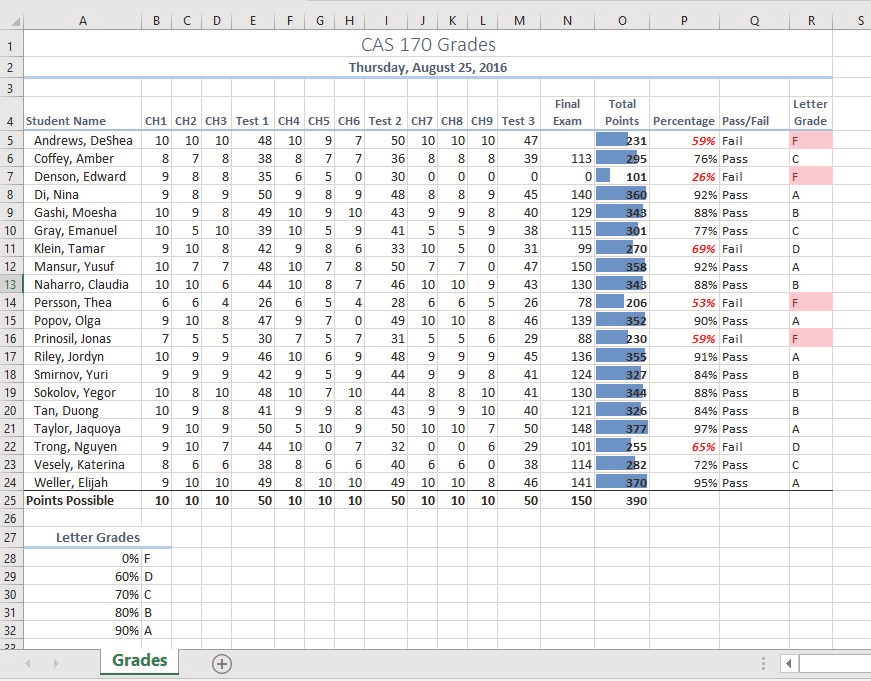
\includegraphics[width=\maxwidth{.95\linewidth}]{gfx/ch03_fig01}
	\caption{Completed Gradebook Worksheet}
	\label{03:fig01}
\end{figure}

\section{More on Formulas and Functions}

\begin{center}
	\begin{objbox}{Learning Objectives}
		\begin{itemize}
			\setlength{\itemsep}{0pt}
			\setlength{\parskip}{0pt}
			\setlength{\parsep}{0pt}
			
			\item Review the use of the \formatfunc{=MAX} function.
			\item Examine the Quick Analysis Tool to create standard calculations, formatting, and charts very quickly.
			\item Create Percentage calculation.

			\begin{itemize}
				\setlength{\itemsep}{0pt}
				\setlength{\parskip}{0pt}
				\setlength{\parsep}{0pt}

				\item Use the Smart Lookup tool to acquire additional information about percentage calculations.
				\item Review the use of Absolute cell reference in a division formula.
			\end{itemize}

		\end{itemize}
	\end{objbox}
\end{center}

\subsection{Another Use for =MAX}

Before we move on to the more interesting calculations we will be discussing in this chapter, we need to determine how many points it is possible for each student to earn for each of the assignments. This information will go into Row 25. The \formatfunc{=MAX} function is our tool of choice.

\textit{Data File: CH3 Data}

\begin{enumerate}
	\item Open the data file \textbf{CH3 Data} and save the file to your computer as \textbf{CH3 Gradebook}.
	\item Make \textsf{B25} the active cell.
	\item Start typing \formatfunc{=MAX} (See Figure \ref{03:fig02}). Note the explanation you see on the offered list of functions. You can either keep typing '(' or double click \textit{MAX} from the list.
\end{enumerate}

\begin{figure}[H]
	\centering
	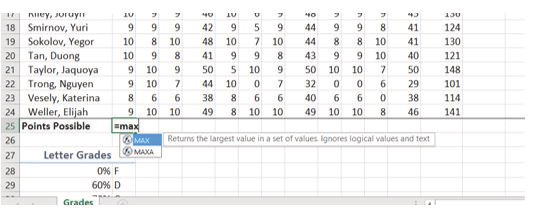
\includegraphics[width=\maxwidth{.95\linewidth}]{gfx/ch03_fig02}
	\caption{Entering a function}
	\label{03:fig02}
\end{figure}

\begin{enumerate}[resume]
	\item Select the range of numbers above row 25. Your calculation will be: \formatfunc{=MAX(B5:B24)}
	\item Now, use the Fill Handle to copy the calculation from Column B through Column N. Note that as you copy the calculation from one column to the next, the cell references change. The calculation in column B reads: \formatfunc{=MAX(B5:B24)}. The one in column N reads \formatfunc{=MAX(N5:N24)}. These cell references are relative references.
\end{enumerate}

By default, the calculations that Excel copies change their cell references relative to the row or column they are copied to. That makes sense. Column N should not display an answer that uses the values in column L.

If you want to see all the calculations you have just created, press \keystroke{Ctrl} + \keystroke{$ \sim $} (See Figure \ref{03:fig03}) \keystroke{Ctrl} + \keystroke{$ \sim $} displays the calculations (formulas). Pressing \keystroke{Ctrl} + \keystroke{$ \sim $} a second time will display calculations in the default view --- as values.

\begin{figure}[H]
	\centering
	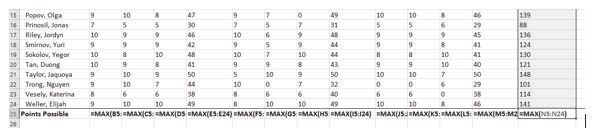
\includegraphics[width=\maxwidth{.95\linewidth}]{gfx/ch03_fig03}
	\caption{Relative References – Displayed as calculations.}
	\label{03:fig03}
\end{figure}

\subsection{Quick Analysis Tool}

The Quick Analysis Tool allows you to create standard calculations, formatting, and charts very quickly. In this exercise we will use it to insert the Total Points for each student in Column O.

Be sure to press \keystroke{Ctrl} + \keystroke{$ \sim $} to return your spreadsheet to the normal view (the formula results should display, not the formulas themselves).

\begin{enumerate}
	\item Select the range of cells \textsf{B5:N25}
	\item In the lower right corner of your selection, you will see the Quick Analysis tool (see Figure \ref{03:fig04}).
\end{enumerate}

\begin{figure}[H]
	\centering
	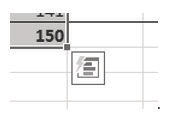
\includegraphics[width=\maxwidth{.95\linewidth}]{gfx/ch03_fig04}
	\caption{Quick Analysis Tool}
	\label{03:fig04}
\end{figure}

\begin{enumerate}[resume]
	\item When you click on it, you will see that there are a number of different options. This time we will be using the Totals option. In future exercises, we will use other options.
	\item Select Totals, and then the SUM option that highlights the right column (see Figure \ref{03:fig05}). Selecting that SUM option places \formatfunc{=SUM()} calculations in column O.
\end{enumerate}

\begin{figure}[H]
	\centering
	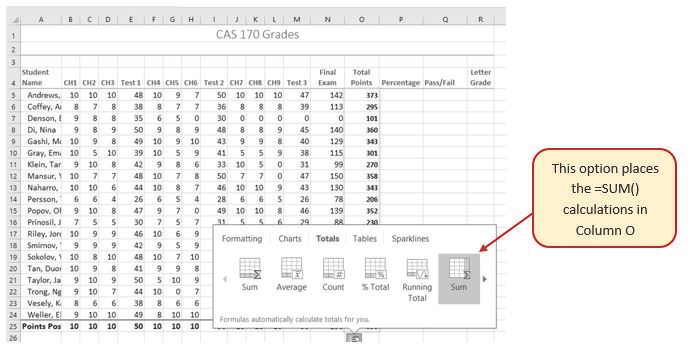
\includegraphics[width=\maxwidth{.95\linewidth}]{gfx/ch03_fig05}
	\caption{Quick Analysis Tool – Totals, Sum Column}
	\label{03:fig05}
\end{figure}

\subsection{Percentage Calculation}

Column P requires a Percentage calculation. Before we launch in to creating a calculation for this, it might be handy to know precisely what it is we are looking for. If you are connected to the internet and are using Excel 2016, you can use the Smart Lookup tool to get more information.

\begin{enumerate}
	\item Select cell \textsf{P4}.
	\item Find the \textbf{Smart Lookup} tool on the \textbf{Review} tab (see Figure \ref{03:fig06}).
	\item Press the \textbf{Smart Lookup} tool to find more about Percentage calculations. If this is the first time you have used the Smart Lookup tool, you may need to respond to a statement about your privacy. Press the \textbf{Got it} button.
\end{enumerate}

I think the first Wikipedia article does a pretty good job explaining the calculation, don't you?

\begin{figure}[H]
	\centering
	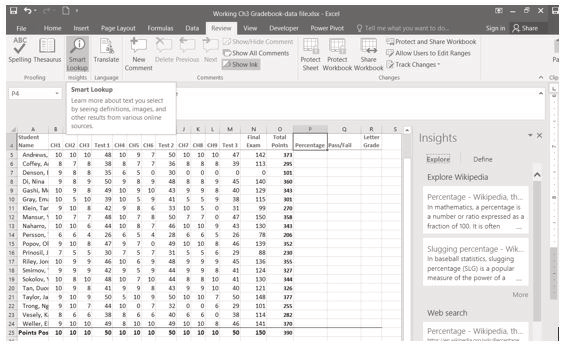
\includegraphics[width=\maxwidth{.95\linewidth}]{gfx/ch03_fig06}
	\caption{Smart Lookup tool}
	\label{03:fig06}
\end{figure}

Now that we know what is needed for the Percentage calculation, we can have Excel do the calculation for us. We need to divide the \textbf{Total Points} for each student by the \textbf{Total Points} of all the \textbf{Points Possible}. Notice that there is a different number on each row for each student. But, there is only one \textbf{Total Points Possible} --- the value that is in cell \textsf{O25}.

1. Make sure that P5 is your active cell.
2. Press = then select cell O5. Press /, then cell O25. Your calculation should look like this: =O5/O25. The result of the formula should be 0.95641026. (So far, so good. DeShea Andrews is doing well in this class – with a percentage grade of almost 96\%. Definitely an ``A''!)
3. Next use the Fill handle to copy the calculation down through row 24 to calculate the other students' grades. You should get the error message $ \#DIV/0! $. This error message reminds us that you cannot divide a number by $ 0 $ (zero). The calculation in \textsf{P9} reads $ =O9/O29 $. The first cell reference is correct --- it points to Moesha Gashi's total points for the class. But the second reference is wrong. It points to an empty cell, \textsf{O29}.

Before copying the calculation, we have to make the second reference (\textsf{O25}) an absolute cell reference. That way, when we copy the formula down, the cell reference for \textsf{O25} will be locked and will not change.

\begin{enumerate}
	\item Make \textsf{P5} the active cell. In the Formula Bar click on O25 (see Figure \ref{03:fig07}).
	\item Press \keystroke{F4} (on the function keys at the top of your keyboard). That will make the \textsf{O25} reference absolute. It will not change when you copy the calculation (see Figure \ref{03:fig08}). (If you are working on a laptop and do not have an \keystroke{F4} function key, you can type in a \$ before the \textsf{O} and another one before the \textsf{25}.)
	\item The calculation now looks like \formatfunc{=O5/\$O\$25}.
	\item Use the Fill Handle to copy the formula down through \textsf{P24} again. Now the formula has the correct values for all students.
\end{enumerate}

\begin{figure}[H]
	\centering
	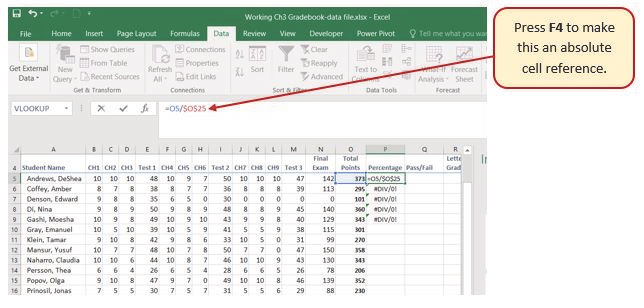
\includegraphics[width=\maxwidth{.95\linewidth}]{gfx/ch03_fig07}
	\caption{Editing a formula}
	\label{03:fig07}
\end{figure}

\begin{figure}[H]
	\centering
	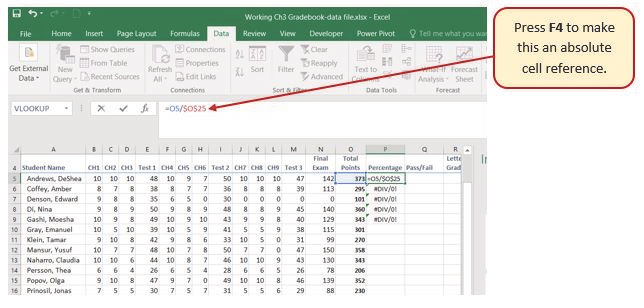
\includegraphics[width=\maxwidth{.95\linewidth}]{gfx/ch03_fig08}
	\caption{Absolute Cell reference – press F4}
	\label{03:fig08}
\end{figure}

Those long decimals are a bit nonstandard so they should be changed to a percent by applying cell formatting.

\begin{enumerate}
	\item Select the range \textsf{P5:P24}.
	\item On the Home tab, in the Number Group, select the \% (Percent Style) button.
\end{enumerate}

\begin{center}
	\begin{sklbox}{Skill Refresher}
		\textbf{Absolute References}
		\\
		\begin{itemize}
			\setlength{\itemsep}{0pt}
			\setlength{\parskip}{0pt}
			\setlength{\parsep}{0pt}

			\item Click in front of the column letter of a cell reference in a formula or function that you do not want altered when the formula or function is pasted into a new cell location.
			\item Press the \keystroke{F4} key or type a dollar sign (\$) in front of the column letter and row number of the cell reference.
						
		\end{itemize}
	\end{sklbox}
\end{center}

\begin{center}
	\begin{tkwbox}{Key Take-Aways}
		\textbf{Functions}
		\\
		\begin{itemize}
			\setlength{\itemsep}{0pt}
			\setlength{\parskip}{0pt}
			\setlength{\parsep}{0pt}

			\item Functions can be created using cell ranges or selected cell locations separated by commas. Make sure you use a cell range (two cell locations separated by a colon) when applying a statistical function to a contiguous range of cells.
			\item To prevent Excel from changing the cell references in a formula or function when they are pasted to a new cell location, you must use an absolute reference. You can do this by placing a dollar sign (\$) in front of the column letter and row number of a cell reference or by using the \keystroke{F4} function key.
			\item The $ \#DIV/0 $ error appears if you create a formula that attempts to divide a constant or the value in a cell reference by zero.
			
		\end{itemize}
	\end{tkwbox}
\end{center}

\section{Logical and Lookup Functions}

\begin{center}
	\begin{objbox}{Learning Objectives}
		\begin{itemize}
			\setlength{\itemsep}{0pt}
			\setlength{\parskip}{0pt}
			\setlength{\parsep}{0pt}

			\item Use an \formatfunc{IF} Function to make logical comparisons between a value and what you expect.
			\item Create a \formatfunc{VLOOKUP} calculation to look up information in a table.
			\item Understand error messages.
			\item Understand how to enter and format Date/Time Functions.
			
		\end{itemize}
	\end{objbox}
\end{center}

In addition to doing arithmetic, Excel can do other kinds of functions based on the data in your spreadsheet. In this section we will use an \formatfunc{=IF} function to determine whether a student is passing or failing the class. Then, we will use a \formatfunc{=VLOOKUP} function to determine what grade each student has earned.

\subsection{If Function}

The \formatfunc{IF} function is one of the most popular functions in Excel. It allows you to make logical comparisons between a value and what you expect. In its simplest form, the \formatfunc{IF} function says something like, ``If the value in a cell is what you expect (true) then do this; otherwise do that.

The \formatfunc{IF} function has three arguments.

\begin{itemize}
	\item \textbf{Logical test}. this is the test to see if the value in a selected cell is what was expected. A test can be something like ``$ B7=14 $'' or ``$ B7>12 $'' or ``$ B7<6 $.''
	\item \textbf{Value\_if\_true}. What to do if the requirements in the logical test are met, for example, if \textsf{B7} is equal to $ 14 $. For this argument you can type text like ``True,'' or ``On budget!'' Or you could insert a calculation, like $ B7*2 $. That is, if \textsf{B7} equals $ 14 $ then multiply it by $ 2 $. Or, if Excel should put nothing at all in the cell then type ``'' (two quotes).
	\item \textbf{Value\_if\_false}. What to do if the requirements in the logical test are \textit{NOT} met; for example, if \textsf{B7} does \textit{NOT} equal $ 14 $. To have Excel do nothing, then type empty double quotes. Of course, Excel can also enter whatever text or calculation is desired.
\end{itemize}

In column Q we would like Excel to tell us whether a student is passing or failing the class. Student who score $ 70\% $ or better will pass the class; but scores less than $ 70\% $ are failing.

\begin{enumerate}
	\item Make sure that \textsf{Q5} is the active cell.
	\item On the Formulas tab, in the Function Library, find the \formatfunc{IF} function on the Logical pulldown menu (see Figure \ref{03:fig09}).
\end{enumerate}

\begin{figure}[H]
	\centering
	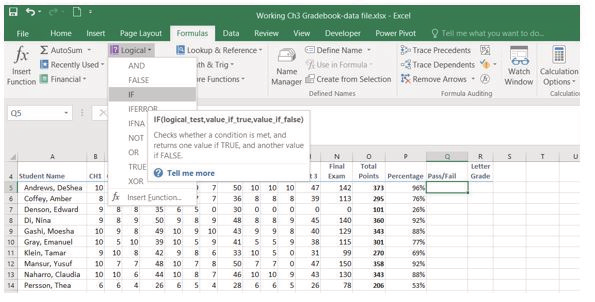
\includegraphics[width=\maxwidth{.95\linewidth}]{gfx/ch03_fig09}
	\caption{IF Function}
	\label{03:fig09}
\end{figure}

Now you will see the \formatfunc{IF} Function dialog box, with a place to enter each of the three arguments.

\begin{enumerate}
	\item Click in the box for \textbf{Logical Test}. To test whether a student's score is less than $ 0.7 $ enter \formatfunc{P5<0.7}.
	\item Click in the box for \textbf{Value\_if\_true}. If the student's score is less than $ 0.7 $, then they are failing the class. In this box, type \textbf{Fail}.
	\item Click in the box for \textbf{Value\_if\_false}. If the student's score is \textit{NOT} less than $ 0.7 $, then they are passing the class. In this box, type \textbf{Pass}.
	\item Make sure that the dialog box matches Figure \ref{03:fig10}.
\end{enumerate}

\begin{figure}[H]
	\centering
	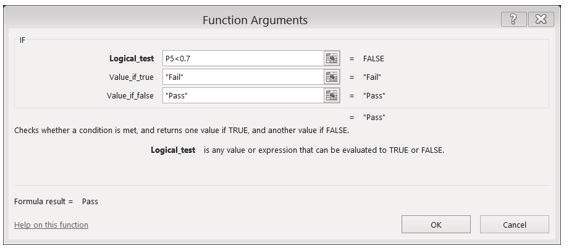
\includegraphics[width=\maxwidth{.95\linewidth}]{gfx/ch03_fig10}
	\caption{IF Function Dialog Box}
	\label{03:fig10}
\end{figure}

Notice that as each box is filled Excel offers a brief explanation of the contents (in the middle below the boxes.) In the lower left hand corner is the results of the calculation. In this case, DeShae is passing the class. Below that is a link to Help on this function. Selecting this link will open Excel help for this function, along with detailed information on how it works.

\begin{enumerate}[resume]
	\item Once the required arguments are entered and checked, press OK. The text ``Pass'' should be displayed in \textsf{Q5} because DeShae is passing the class.
	\item Use the Fill handle to copy the \formatfunc{IF} function down through row 24.
	\item Click on \textsf{Q5}. The formula bar should display the \formatfunc{IF} calculation: \formatfunc{=IF(P5<0.7,''Fail'',''Pass'')} (see Figure \ref{03:fig11}).
\end{enumerate}

\begin{figure}[H]
	\centering
	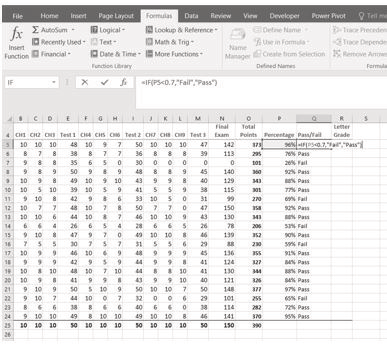
\includegraphics[width=\maxwidth{.95\linewidth}]{gfx/ch03_fig11}
	\caption{IF Function Results}
	\label{03:fig11}
\end{figure}

\subsection{Vlookup Function}

A \formatfunc{VLOOKUP} function is used to look up information in a table. Sometimes that table is on a different sheet in the workbook, though it can be in another file entirely. In this case, all students' grades are determined on their percentage score. The table that defines the scores and the grades is in \textsf{A28:B32}.

There are four pieces of information that needed to build the \formatfunc{VLOOKUP} syntax. 

\begin{itemize}
	\item The value to look up, also called the \textbf{Lookup\_value}. In lthe example, the lookup value will be the student's percentage score in column P.
	\item The \textbf{Table\_array} is the range (table) where the lookup values are located. In this example the table of percentages and corresponding letter grades is in the range \textsf{A28:B32}. The lookup value should always be in the first column in the table array for \formatfunc{VLOOKUP} to work correctly. 
	\item The \textbf{Col\_index\_num} is the column number in the range that contains the value to return. In this example, \textsf{A28:B32} is the Table\_array range so column A is the first column (1), column B is the second column (2), and so on if there were other columns. To return the grade in column B, the number 2 would be entered as the Col\_index\_num.
	\item The \textbf{Range\_lookup} is TRUE for an \textit{approximate} match or FALSE for an exact match. If this is left blank the default value will be TRUE, or an approximate match.
\end{itemize}

Follow these steps to create the \formatfunc{VLOOKUP} to display the correct Letter Grade in column R.

\begin{enumerate}
	\item Make sure that \textsf{R5} is the active cell.
	\item On the Formulas tab in the Function Library, find the \formatfunc{VLOOKUP} function on the Lookup \& Reference pull-down menu (see Figure \ref{03:fig12}).
\end{enumerate}

\begin{figure}[H]
	\centering
	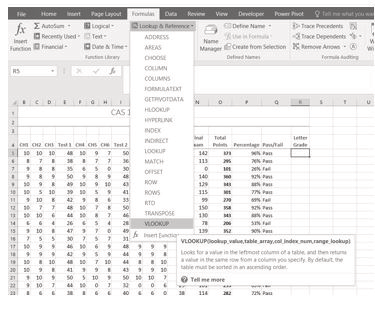
\includegraphics[width=\maxwidth{.95\linewidth}]{gfx/ch03_fig12}
	\caption{VLOOKUP Function}
	\label{03:fig12}
\end{figure}

Fill in the dialog box so that it looks like Figure \ref{03:fig13}.

\begin{itemize}
	\item \textbf{Lookup\_value}. Specify the percentage score, which is in cell \textsf{P5} for the first student.
	\item \textbf{Table\_array}. This is the range that contains the value to be returned by the function. In this case, that range is \textsf{A28:B32}. Note that this range does \textit{NOT} include the label in row 27; just the actual data. The cell references for the Table\_array need to be absolute: \textsf{\$A\$28:\$B\$32}. When this function is copied to other cells the cell references should not change.
	\item \textbf{Col\_index\_number}. This is the column in the table array range that includes the information that should be returned. In this case, the grades are in the 2nd column of the range so the column index will be $ 2 $.
	\item \textbf{Range\_lookup}. Since an approximate match is appropriate for this application the default value of TRUE is acceptable, so do not enter anything for this argument.
\end{itemize}

\begin{enumerate}[resume]
	\item Be sure to observe the helpful definitions that Excel offers while filling in the \formatfunc{VLOOKUP} dialog box.
	\item When the dialog box is complete, press OK.
	\item The calculation in the formula bar is: \formatfunc{=VLOOKUP(P5,\$A\$28:\$B\$32,2)}
	\item Use the fill handle to copy the function down through row $ 24 $. The results displayed should match Figure \ref{03:fig13}.
\end{enumerate}

\begin{figure}[H]
	\centering
	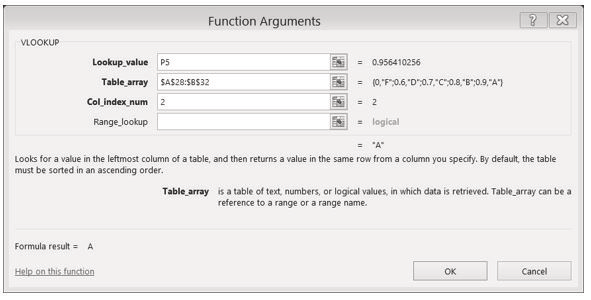
\includegraphics[width=\maxwidth{.95\linewidth}]{gfx/ch03_fig13}
	\caption{VLOOKUP completed dialog box}
	\label{03:fig13}
\end{figure}

\begin{figure}[H]
	\centering
	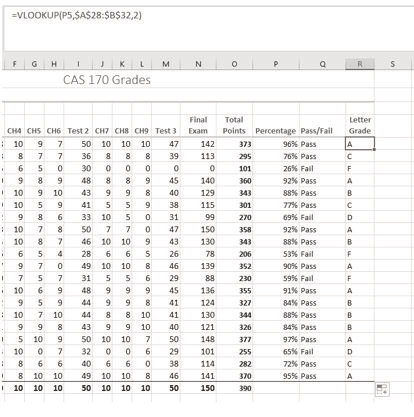
\includegraphics[width=\maxwidth{.95\linewidth}]{gfx/ch03_fig14}
	\caption{VLOOKUP Complete}
	\label{03:fig14}
\end{figure}

What if the \formatfunc{VLOOKUP} function does not work as expected? In this case, a mistake was made in either the calculation of the \% scores or there is an error in the \formatfunc{VLOOKUP} function. To make repairs to the function, make sure that \textsf{R5} is the active cell. On the Formula bar, press the Insert Function button (see Figure \ref{03:fig15}). That will reopen the dialog box to make repairs. A common error is to forget to make the cell references for the Table\_array absolute. Press OK when the correction is completed and then recopy the corrected function.

\begin{figure}[H]
	\centering
	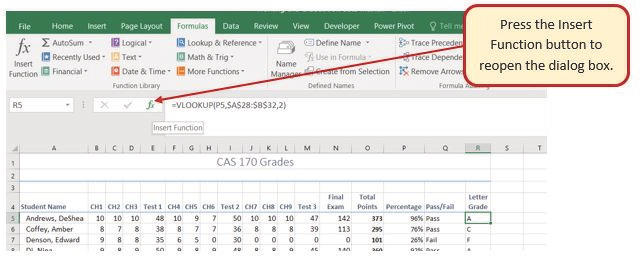
\includegraphics[width=\maxwidth{.95\linewidth}]{gfx/ch03_fig15}
	\caption{Insert Function}
	\label{03:fig15}
\end{figure}

\subsection{Error Messages}

Sometimes Excel notices errors in the calculations and may post a slightly mysterious error message. A list of common error messages can be found in Table \ref{03:tab01}.

{\small
	\begin{longtable}{p{0.75in}p{3.50in}} %Max width: 4.25in
		\textbf{Message} & \textbf{What Went Wrong} \endhead
		\hline \\
		$ \#DIV/0! $ & The division operation refers to a cell that contains the value $ 0 $ or is blank.\\
		\#N/A & Technically, this is not an error value but a special value 		that can be manually entered into a cell to indicate that there is no value yet. This is a placeholder used while a spreadsheet is being developed.\\
		\#NAME? & This error value appears when a range name is incorrectly entered or the name is deleted. Also, this commonly means that the formula is missing quotation marks around a text string.\\
		\#NULL & This error occurs if a space used instead of a comma between ranges in function arguments. The formula needs to be carefully checked and corrected.\\
		\#NUM & This error is caused by an invalid argument in an Excel	function or by a formula that produces a number too large or too small for the worksheet.\\
		\#REF & This error occurs when a cell referred to in a formula has been deleted.\\
		\#VALUE & This error is most often the result of specifying a mathematical operation that refers to one or more cells that contain text.\\
		\caption{Common Error Messages}
		\label{03:tab01}
	\end{longtable}
}

\footnote{Table \ref{03:tab01} was adapted from  \url{https://www.dummies.com/software/microsoft-office/excel/understanding-excel-2010s-formula-error-values/}}

\subsection{Date Functions}

Very often dates and times are an important part of Excel data. Numbers that are correct today may not be accurate tomorrow so it is frequently useful to include dates and times on your spreadsheets.

These dates and times fall into two categories.

\begin{itemize}
	\item \textbf{Remain the same.} For instance, if a spreadsheet includes data for May 15th then that date should not change each time the spreadsheet is accessed.
	\item \textbf{Change to reflect the current date/time.} When it is important to have the current date or time on a spreadsheet then Excel should update the information regularly.
\end{itemize}

Take a look at the list of Date and Time functions offered in the Function Library on the Formulas tab (see Figure \ref{03:fig16}).

\begin{figure}[H]
	\centering
	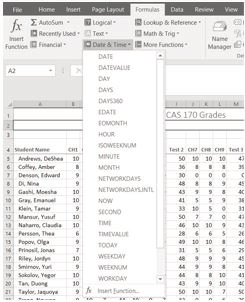
\includegraphics[width=\maxwidth{.95\linewidth}]{gfx/ch03_fig16}
	\caption{Date \& Time Functions}
	\label{03:fig16}
\end{figure}

For the gradebook, the date and time should be displayed in \textsf{A2}, and it needs to be updated whenever the workbook file is opened.

\begin{enumerate}
	\item Make \textsf{A2} your active cell. Notice that \textsf{A2} extends all the way from column A to Column R. Previously, someone has used the Merge \& Center tool on this cell to make it match the title above.
	\item On the Formulas tab, in the Function Library, select \formatfunc{NOW} from the Date \& Time drop-down list and then click OK.
	\item The result in the formula bar is: \formatfunc{=NOW()} and the result in \textsf{A2} depends on the current date and time. The \formatfunc{NOW} function is a very handy function, it takes no arguments and is volatile! That is not as alarming as it may seem. This just means that it doesn't need any information to do its job and the results will change frequently. 
	\item Make sure that \textsf{A1} is your active cell and press  \keystroke{F9} to update the time.
\end{enumerate}

Excel will update this field independently whenever the file is saved, reopened, or printed. It may happen more frequently than that, depending on how the Excel installation was set up.

Another variation of the current date is the \formatfunc{TODAY} function.

\begin{enumerate}
	\item Make sure \textsf{A2} is the active cell. Press \keystroke{Delete} to remove the \formatfunc{NOW} function.
	\item From the Date \& Time drop-down list in the Function Library on the Formulas tab (see Figure \ref{03:fig16}), select \formatfunc{TODAY} and then click OK.
	\item The result in the formula bar is \formatfunc{=TODAY()} and the result in \textsf{A2} is the current date. Since the time was not requested it is likely 12:00. That is not very helpful so the date format needs to be adjusted.
	\item On the Home tab, in the Number group, press the Number Format Launch button (see Figure \ref{03:fig17}).
	\item In the \textbf{Format Cells} dialog box, click the Number tab. Choose the \textbf{Date} category and select \textit{Wednesday, March 14, 2012} (this format is called \textbf{Long Date}).
	\item The current day and date should now be displayed in \textsf{A2}.
\end{enumerate}

\begin{figure}[H]
	\centering
	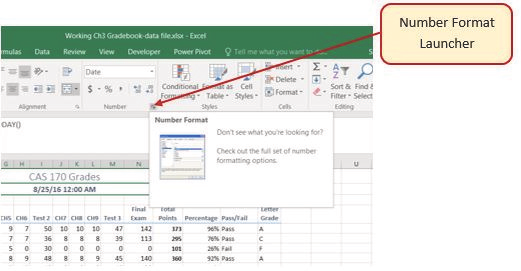
\includegraphics[width=\maxwidth{.95\linewidth}]{gfx/ch03_fig17}
	\caption{Number Format Launcher}
	\label{03:fig17}
\end{figure}

\begin{center}
	\begin{shtcutbox}{Keyboard Shortcuts}
		\textbf{Static Date and Time}
		\\
		\begin{itemize}
			\setlength{\itemsep}{0pt}
			\setlength{\parskip}{0pt}
			\setlength{\parsep}{0pt}

			\item \keystroke{CTRL} + \keystroke{;} (semicolon) inserts the current date
			\item \keystroke{CTRL} + \keystroke{:} (colon) inserts the current time.
			
		\end{itemize}
	\end{shtcutbox}
\end{center}


\begin{center}
	\begin{tkwbox}{Key Take-Aways}
		\textbf{Date Functions}
		\\
		\begin{itemize}
			\setlength{\itemsep}{0pt}
			\setlength{\parskip}{0pt}
			\setlength{\parsep}{0pt}

			\item Functions don't always have to be about arithmetic. Excel provides functions that will help you perform logical evaluations, look things up, and work with dates and times.
			\item Excel displays error messages when your formulas and functions are not constructed properly.
			
		\end{itemize}
	\end{tkwbox}
\end{center}

\section{Conditional Formatting}

\begin{center}
	\begin{objbox}{Learning Objectives}
		\begin{itemize}
			\setlength{\itemsep}{0pt}
			\setlength{\parskip}{0pt}
			\setlength{\parsep}{0pt}

			\item Use Conditional Formatting techniques to provide flexible highlighting or applying specified formatting only when certain conditions are met. Techniques include:

			\begin{itemize}			
				\item \textbf{Data bars}. Makes it easy to visualize values in a range of cells.
				\item \textbf{Cell Rules}. Highlights values that match the requirements you specify.
			\end{itemize}

		\end{itemize}
	\end{objbox}
\end{center}

All necessary calculations are now in the CAS 170 Grades spreadsheet. However, the grade book contains a lot of data. To make it easier to quickly find the most important pieces of data, Excel provides \textit{Conditional Formatting}.

\begin{enumerate}
	\item Select the values in the Total Points column (\textsf{O5:O24}).
	\item At the bottom of the selection, click on the Quick Analysis Tool. On the Formatting tab, select Data Bars (see Figure \ref{03:fig18}).
\end{enumerate}

Excel places blue bars on top of the values; long blue bars for larger numbers, shorter ones for smaller numbers. This makes it easier to see how well each student did in the class without having to look at the specific numbers.

\begin{figure}[H]
	\centering
	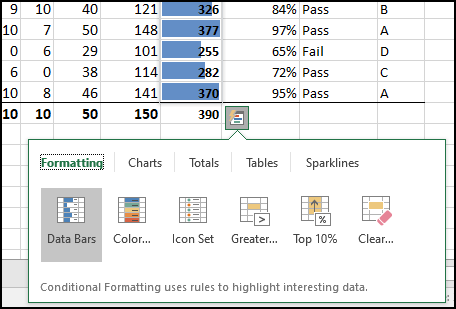
\includegraphics[width=\maxwidth{.95\linewidth}]{gfx/ch03_fig18}
	\caption{Data Bars on the Quick Analysis tool}
	\label{03:fig18}
\end{figure}


Following is another way to apply Data Bars.

\begin{enumerate}
	\item Select the range that needs data bars
	\item On the Home tab, in the Styles group, select Data Bars from the Conditional Formatting tool.
	\item From there you can select data bars of different colors and opacities (see Figure \ref{03:fig19}).
\end{enumerate}

\begin{figure}[H]
	\centering
	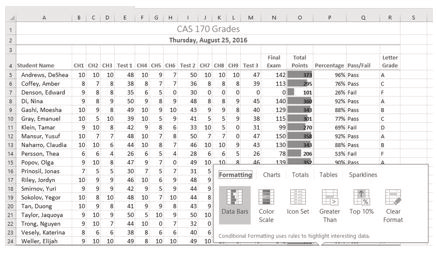
\includegraphics[width=\maxwidth{.95\linewidth}]{gfx/ch03_fig19}
	\caption{Data Bars on the Conditional Formatting tool}
	\label{03:fig19}
\end{figure}

It is even more important to highlight the students who are failing in the class, so that will be done in two places, the Percentages and Letter Grade columns. To start, any \textbf{F} letter grades should be formatted with a light red fill color and dark red text.

\begin{enumerate}
	\item Select the Letter Grades (\textsf{R5:R24}).
	\item On the Home tab, in the Styles group, select Highlight Cell Rules from the Conditional Formatting tool (see Figure \ref{03:fig20}).
	\item Select \textbf{Equal To}
	\item Fill out the Equal to dialog box so that cells that are equal to \textbf{F} have Light Red Fill with Dark Red Text (see Figure \ref{03:fig21}).
\end{enumerate}

\begin{figure}[H]
	\centering
	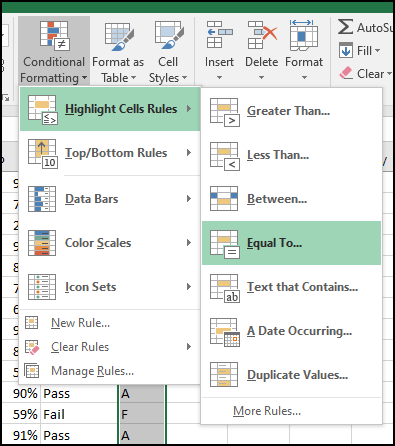
\includegraphics[width=\maxwidth{.95\linewidth}]{gfx/ch03_fig20}
	\caption{Conditional Formatting Equal To}
	\label{03:fig20}
\end{figure}

\begin{figure}[H]
	\centering
	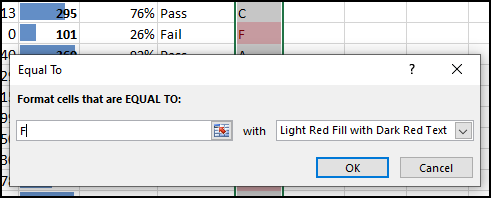
\includegraphics[width=\maxwidth{.95\linewidth}]{gfx/ch03_fig21}
	\caption{Conditional Formatting Equal To Dialog Box}
	\label{03:fig21}
\end{figure}

Now, highlight students who are passing the class. This time, use the Pass/Fail text in the Pass/Fail column. If the text for a student is ``Pass'' the cell should be formatted with a yellow fill with dark yellow text.

\begin{enumerate}
	\item Select the Pass/Fail grades (\textsf{Q5:Q24}).
	\item On the Home tab, in the Styles group, select Highlight Cell Rules from the Conditional Formatting tool (see Figure \ref{03:fig20}).
	\item Select \textbf{Equal To} 
	\item Fill out the Equal to dialog box so that cells that are equal to ``Pass'' have Yellow Fill with Dark Yellow Text. (To find the Yellow Fill with Dark Yellow text option, click the the down arrow at the end of the last (with) box).
\end{enumerate}

The default styles are a simple way to make specified data stand out, but any cell formatting can be set. When using custom cell formatting, it is probably a good idea to include other styling in addition to color. Remember that spreadsheets are often printed in black and white so Conditional formatting that relies only on color would be lost. Next, use conditional formatting to display any Percentages that are less than $ 60\% $ with red text formatted in bold and italic.

\begin{enumerate}
	\item Select the Percentage grades (\textsf{P5:P24}).
	\item On the Home tab, in the Styles group, select Highlight Cell Rules from the Conditional Formatting tool (see Figure \ref{03:fig20}).
	\item Select \textbf{Less Than}
	\item Fill out the Less Than dialog box so that cells that are less than $ 0.6 $ will be have conditional formatting. Instead of using the default red text on a light red fill, press the down arrow at the end of that box and select \textbf{Custom Format}.
	\item On the Font tab of the Format Cells dialog box, in the Font style box, select \textbf{Bold Italic}. In the Color box, select \textbf{Red} (see Figure \ref{03:fig22}).
	\item Press OK. Then press OK again.
\end{enumerate}

\begin{figure}[H]
	\centering
	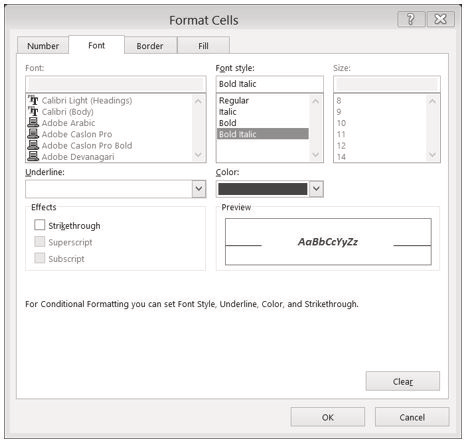
\includegraphics[width=\maxwidth{.95\linewidth}]{gfx/ch03_fig22}
	\caption{Conditional Formatting Custom Format Cells Dialog box}
	\label{03:fig22}
\end{figure}

Conditional Formatting is valuable in that it reflects the current data and it changes to whenever the data changes. To test this, delete DeShea's final exam score. (Select \textsf{N5}. Press Delete on your keyboard.) Suddenly, DeShae is failing the course and the Conditional Formatting reflects that. Press CTRL Z (Undo). The test score reappears and the Conditional formatting reflects that as well.

\subsection{Making Changes}

What if there is a mistake with the Conditional Formatting or it needs to be delete altogether? Use the \textbf{Conditional Formatting Manage Rules} tool. In the grade book example, remove the conditional formatting rule that formats the ``Pass'' text with yellow and modify the minimum passing percentage.

\begin{enumerate}
	\item On the Home Tab, in the Styles Group, select \textbf{Manage Rules} at the very bottom of the Conditional Formatting drop-down list.
	\item Show formatting rules for: \textbf{This Worksheet} (see Figure \ref{03:fig23}).
	\item Since there is no need to highlight the students who are passing the class, select that rule in the Rules Manager and press the \textbf{Delete Rule} button.
\end{enumerate}

\begin{figure}[H]
	\centering
	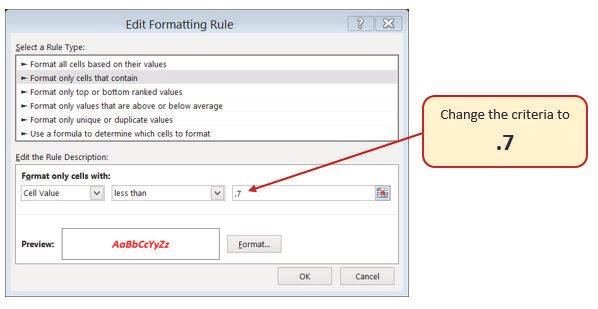
\includegraphics[width=\maxwidth{.95\linewidth}]{gfx/ch03_fig23}
	\caption{Conditional Formatting Manage Rules}
	\label{03:fig23}
\end{figure}

In a previous exercise (the \formatfunc{IF} function), it was decided that students were failing if they got a percentage score of less than $ 70\% $, so the Conditional Formatting rule in the Percentage column needs repair.

\begin{enumerate}[resume]
	\item Select the rule that reads Cell Value $ <0.6 $.
	\item Select the Edit Rule button, and change the $ 0.6 $ to $ 0.7 $ (see Figure \ref{03:fig24}).
	\item Click OK (or Apply) twice. Double check that your completed workbook matches Figure \ref{03:fig25}.
\end{enumerate}

\begin{figure}[H]
	\centering
	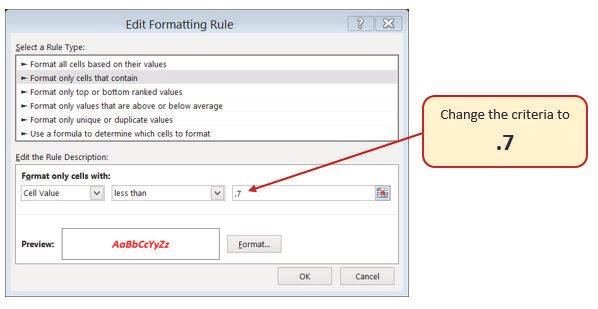
\includegraphics[width=\maxwidth{.95\linewidth}]{gfx/ch03_fig24}
	\caption{Conditional Formatting Edit Formatting Rule Dialog box}
	\label{03:fig24}
\end{figure}

\begin{figure}[H]
	\centering
	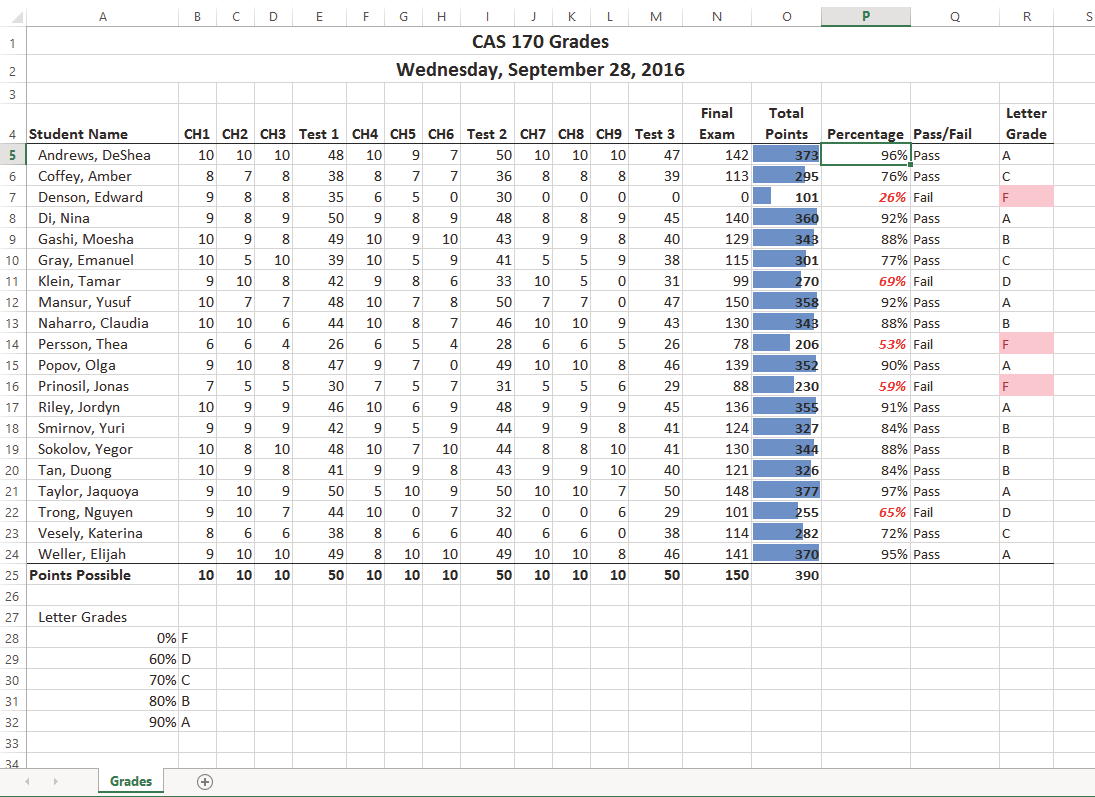
\includegraphics[width=\maxwidth{.95\linewidth}]{gfx/ch03_fig25}
	\caption{Completed Ch3 Gradebook}
	\label{03:fig25}
\end{figure}

\subsection{Setting the Print Area}

Before this workbook is finished, it needs to be prepared for printing. The first thing to do is set the Print Area so that the table of Letter Grades in \textsf{A27:B32} does not print.

\begin{enumerate}
	\item Select \textsf{A1:R25}. This is the only part of the worksheet to be printed.
	\item On the \textbf{Page Layout} ribbon, click the \textbf{Print Area} button. Choose \textbf{Set Print Area} from the menu.
\end{enumerate}

Next, preview the worksheet in Print Preview to check that the print area setting worked and to make sure it is printing on one page.

\begin{enumerate}
	\item View the workbook in Print Preview.
	\item Set the page orientation to \textbf{Landscape}.
	\item Change the page scaling if needed so that the entire worksheet prints on one page.
	\item Save and close the \textbf{CH3 Gradebook} workbook.
	\item Compare your work with the self-check answer key (found in the Course Files) and then submit the \textbf{CH3 Gradebook} workbook as directed by the instructor.
\end{enumerate}

\section{Preparing to Print}

\begin{center}
	\begin{objbox}{Learning Objectives}
		\begin{itemize}
			\setlength{\itemsep}{0pt}
			\setlength{\parskip}{0pt}
			\setlength{\parsep}{0pt}

			\item Locate and fix formatting consistency errors.
			\item Apply new formatting techniques.
			\item Use Print Titles to repeat rows and columns on each page of a multiple page worksheet.
			\item Control where page breaks occur in a multiple page worksheet.
			
		\end{itemize}
	\end{objbox}
\end{center}

In this section, a worksheet will be reviewed for formatting consistency. Also, two new formatting techniques are presented. The worksheet used in this section currently prints on four pages, so new page setup options are used to control how these pages print. 

\subsection{Reviewing Formatting for Consistency}

\textit{Download Data File: CH3 PTP Data}

The workbook contains data about the national parks in the western United States. The workbook has been formatted but needs to be reviewed for consistency and prepared for printing. Figure \ref{03:fig26} shows how the second page of the finished worksheet will appear in Print Preview.

\begin{figure}[H]
	\centering
	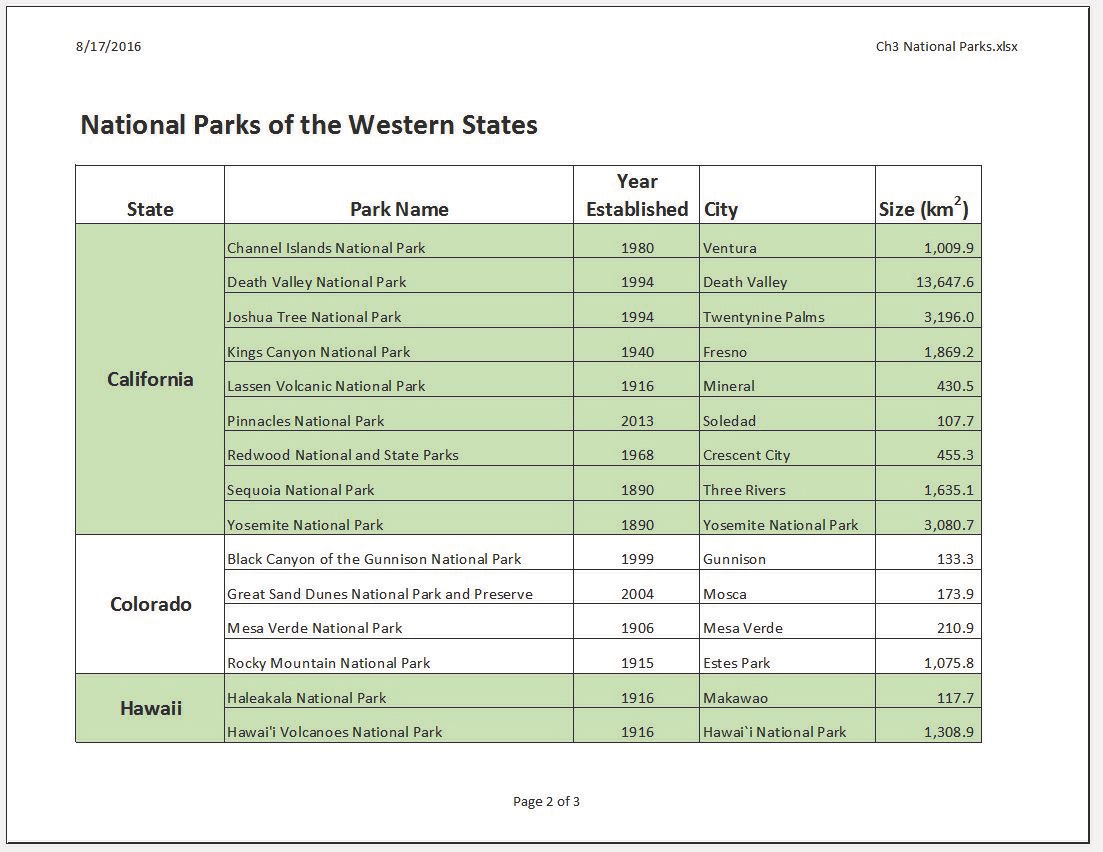
\includegraphics[width=\maxwidth{.95\linewidth}]{gfx/ch03_fig26}
	\caption{Completed National Parks worksheet}
	\label{03:fig26}
\end{figure}

\subsection{Reviewing Formatting for Inconsistencies}

The first thing to do is review the worksheet for formatting inconsistencies.

\begin{enumerate}
	\item Open the data file named \textbf{CH3 PTP Data} and use the File/Save As command to save it with the new name \textbf{CH3 National Parks}.
	\item Scroll through the worksheet and locate the following formatting errors.

	\begin{itemize}
		\item The formatting of the Utah label does not match the other states.
		\item The Year Established values for Hawaii are not center aligned like the other years.
		\item The cells for the Nevada data should have the same green fill color as the other alternating states.
		\item The number of digits after the decimal place for the Size values is inconsistent. Also, these values should be formatted with Comma style to make them easier to read.
	\end{itemize}

		\item To fix these errors, complete the following steps.

	\begin{itemize}
		\item Merge \& Center \textsf{A34:A38}. Change the font size to 16 and apply Bold format.
		\item Center align \textsf{C28:C29}.
		\item Apply the green fill color to \textsf{A31:E31} (be sure to match the green fill color of the other states).
		\item Select \textsf{E4:E43} and apply Comma Style. Use Increase Decimal and/or Decrease Decimal until one digit appears after the decimal place for all values.
	\end{itemize}
	
	\item While these formatting errors are being corrected all typos should also be corrected.
\end{enumerate}

\subsection{Fine-Tuning Formatting}

Now that the formatting inconsistencies have been corrected, apply additional formatting techniques to make the worksheet look better. Start by vertically aligning the names of the states within the cells.

\begin{enumerate}
	\item Select \textsf{A4:A43} (the cells with the state labels).
	\item Click the Home tab on the ribbon.
	\item In the Alignment group, click the \textbf{Middle Align} button (see Figure \ref{03:fig27}). Notice that the names of the states are now centered between the top and bottom borders of the cells.
\end{enumerate}

\begin{figure}[H]
	\centering
	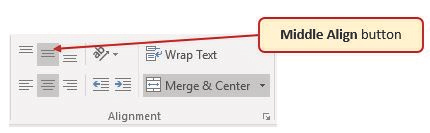
\includegraphics[width=\maxwidth{.95\linewidth}]{gfx/ch03_fig27}
	\caption{Alignment Group}
	\label{03:fig27}
\end{figure}

The next formatting correction is to change the label in \textsf{E3} from ``Size (km2)'' to ``Size (km\textsuperscript{2})'' with the $ 2 $ after km formatted as a superscript.

\begin{enumerate}
	\item Double-click on cell \textsf{E3} to enter Edit mode
	\item Select just the $ 2 $ (be careful not to select anything else).
	\item On the ribbon (Home tab) click the dialog box launcher arrow in the Font group.
	\item In the Effects section of the Format Cells dialog box, check the box for Superscript (see Figure \ref{03:fig28}). Click OK.
	\item Save the \textbf{CH3 National Parks} file.
\end{enumerate}

\begin{figure}[H]
	\centering
	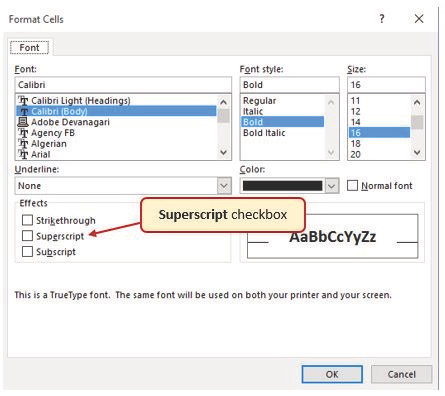
\includegraphics[width=\maxwidth{.95\linewidth}]{gfx/ch03_fig28}
	\caption{Font Tab in Format Cells Dialog Box}
	\label{03:fig28}
\end{figure}

\subsection{Repeating Column (And Row) Labels}

Now that the cell and text formatting are corrected, review the worksheet in Print Preview. Notice that the worksheet is printing on multiple pages and it is not possible to know what each column of data represents on some of the pages.

\begin{enumerate}
	\item With the \textbf{CH3 National Parks} file still open, go to Backstage View by clicking the File tab on the ribbon. Select Print from the menu.
	\item Click through each of the pages. The worksheet is currently printing on four pages, with the City and Sizes columns printing on separate pages from the rest of the data.
	\item Change the Orientation from Portrait to Landscape to fit all of the columns on one page. Unfortunately, the second and third pages have no column labels to identify the information in each column. Use \textbf{Print Titles} to repeat the first three rows of the worksheet on each of the printed pages. 
	\item Exit Print Preview.
	\item Exit Backstage View then click the Page Layout tab on the ribbon.
	\item Click the Print Titles button in the Page Setup group on the ribbon. The dialog box shown in Figure \ref{03:fig29} should appear.
\end{enumerate}

\begin{figure}[H]
	\centering
	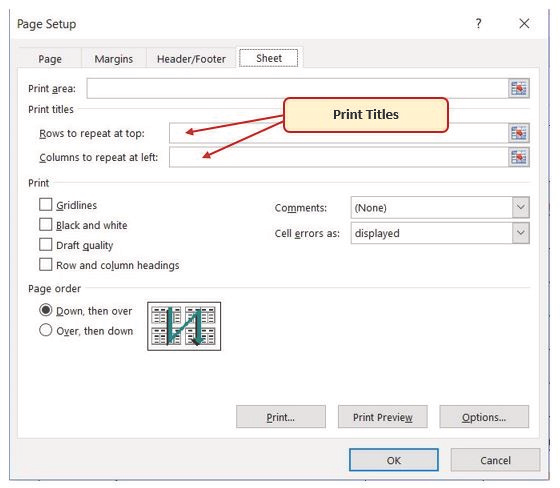
\includegraphics[width=\maxwidth{.95\linewidth}]{gfx/ch03_fig29}
	\caption{Print Titles}
	\label{03:fig29}
\end{figure}

\begin{enumerate}[resume]
	\item Click in the \textit{Rows to repeat at top} box. Be sure the insertion point is blinking in that box before moving on to the next step.
	\item In the worksheet, select Rows 1 through 3. The text \$1:\$3 should now appear in the \textit{Rows to repeat at top} box.
	\item Click OK.
\end{enumerate}

The worksheet does not change in Normal view, so return to Print Preview. While in Print Preview, notice that the pages are breaking in inconvenient places, but that will be corrected in the next section.

\begin{enumerate}
	\item Go to Print Preview and look at each of the pages. Notice that the first three rows are now repeated at the top of each page.
	\item Exit Backstage View.
\end{enumerate}

\begin{center}
	\begin{sklbox}{Skill Refresher}
		\textbf{Creating Print Titles}
		\\
		\begin{itemize}
			\setlength{\itemsep}{0pt}
			\setlength{\parskip}{0pt}
			\setlength{\parsep}{0pt}

			\item Open the Page Setup dialog box and click the Sheet tab.
			\item Click in the Rows to repeat at top: box or the Columns to repeat at left: box.
			\item Click in the worksheet and select the row(s) or column(s) that you want to repeat on each page.
						
		\end{itemize}
	\end{sklbox}
\end{center}

\subsection{Inserting Page Breaks}

Notice that the data for California is split between the first and second pages. Since it is desirable to keep all of the data for each state on the same page, the page breaks need to be adjusted. Start by inserting a page break before the California data to force it to start on the second page, then move the page break for the third page if needed. To make these changes work in \textbf{Page Break Preview}.

\begin{enumerate}
	\item 1. Click the View tab on the ribbon then click \textbf{Page Break Preview} in the Workbook Views Group. Your screen should look similar to Figure \ref{03:fig30}.
\end{enumerate}

\begin{figure}[H]
	\centering
	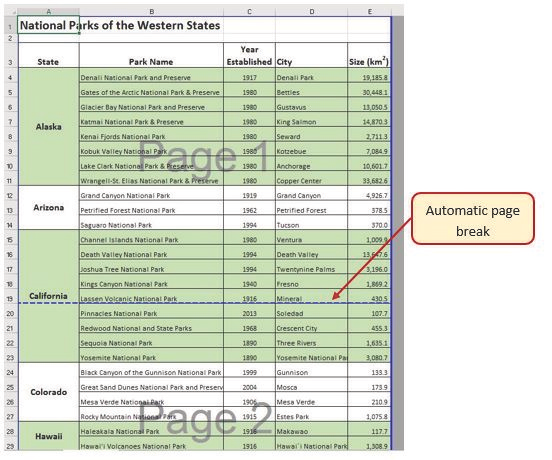
\includegraphics[width=\maxwidth{.95\linewidth}]{gfx/ch03_fig30}
	\caption{Page Break Preview}
	\label{03:fig30}
\end{figure}

In Page Break Preview, automatic page breaks are displayed as dotted blue lines. Notice the dotted blue lines after rows $ 19 $ and $ 35 $. These lines indicate where Excel will start a new page. For this worksheet, the first page should to break at the California data, so insert a manual page break.

\begin{enumerate}
	\item Select cell \textsf{A15}. When inserting a page break, select the cell \textit{below} where you want the page break to appear.
	\item Click the Page Layout tab on the ribbon.
	\item Click the Breaks button in the Page Setup group (see Figure \ref{03:fig31}).
	\item Select \textbf{Insert Page Break} from the menu. There is now a solid blue line after row $ 14 $, which indicates a manual page break was inserted.
	\item Go to Print Preview. Notice that the California data now starts on the second page.
\end{enumerate}

\begin{figure}[H]
	\centering
	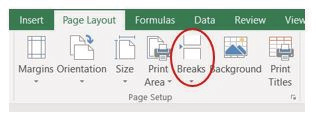
\includegraphics[width=\maxwidth{.95\linewidth}]{gfx/ch03_fig31}
	\caption{Breaks Button on Page Layout tab}
	\label{03:fig31}
\end{figure}

After looking at each page in Print Preview it was decided that the third page should start with Montana. To make this change, move the automatic page break that appears after Nevada.

\begin{enumerate}
	\item Exit Backstage View. Switch back to Page Break Preview if needed.
	\item Locate the next dotted blue line (automatic page break).
	\item Put the pointer over the dotted blue line and it will switch to a vertical double-headed arrow. Click on the dotted blue line and drag it above Montana.
	\item Release the mouse button when the line is above row $ 30 $ (above Montana). The line will now be a solid blue line, indicating a manual page break.
	\item Go to Print Preview. The Montana data now appears at the top of the third page.
\end{enumerate}

While evaluating the pages in Print Preview it appears that there is too much white space at the bottom of the pages. To fix this, center the contents vertically on the pages.

\begin{enumerate}
	\item Click the Page Setup link at the bottom of the Settings section of Backstage View to open the Page Setup dialog box.
	\item Click on the Margins tab.
	\item In the Center on page section, check the box for Vertically then click OK.
	\item Review each page in Print Preview to see the changes. Exit Backstage View.
\end{enumerate}

\subsection{Creating a Header and Footer Using Page Layout View}

Now that the worksheet is printing on three pages, with page breaks in appropriate places, it is time to add a header with the current date and filename. A footer will also be added with the page number and the total number of pages that will appear as ``Page 1 of 3''. 

\begin{enumerate}
	\item Click the View tab on the ribbon and click the Page Layout button in the Workbook Views group.
	\item The white space at the top of the worksheet should say Add header. Place the mouse pointer over the left section of the Header and click to activate that section.
	\item Click the Header \& Footer Tools Design tab on the ribbon.
	\item Click the \textbf{Current Date} button in the Header \& Footer Elements group (see Figure \ref{03:fig32}). Inserting the date this way will insert a field that will update every time the workbook is opened.
	\item Click in the right section of the Header. Click the \textbf{Filename} button in the Header \& Footer Elements group (see Figure \ref{03:fig32}). Inserting the filename this way will insert a field that will update if the filename is changed.
	\item Click the \textbf{Go to Footer} button in the Navigation group of commands.
	\item In the center section of the footer, type the word Page with a space after it.
	\item Click the Page Number button in the Header \& Footer Elements group (see Figure \ref{03:fig32}), then type a space after the \&[Page] code that appears.
	\item Type the word ``of'' with a space after it, then click the \textbf{Number of Pages} button in the Header \& Footer Elements group (see Figure \ref{03:fig32}). The footer should match Figure \ref{03:fig33}.
	\item Click anywhere on the worksheet to close the Footer editing.
	\item Review the worksheet again in Print Preview. Pay careful attention to the page numbers in the footer to ensure they will print correctly, then exit Backstage View.
	\item Save the \textbf{CH3 National Parks} workbook.
	\item Compare your work with the self-check answer key (found in the Course Files) and then submit the \textbf{CH3 National Parks} workbook as directed by your instructor.
\end{enumerate}

\begin{figure}[H]
	\centering
	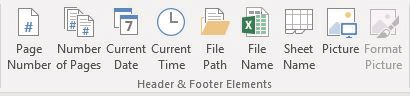
\includegraphics[width=\maxwidth{.95\linewidth}]{gfx/ch03_fig32}
	\caption{Header \& Footer Elements buttons}
	\label{03:fig32}
\end{figure}

\begin{figure}[H]
	\centering
	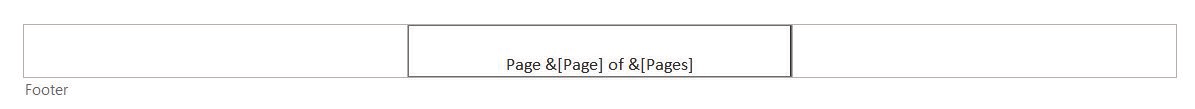
\includegraphics[width=\maxwidth{.95\linewidth}]{gfx/ch03_fig33}
	\caption{Completed Footer}
	\label{03:fig33}
\end{figure}

\begin{center}
	\begin{sklbox}{Skill Refresher}
		\textbf{Inserting Page Numbers}
		\\
		\begin{itemize}
			\setlength{\itemsep}{0pt}
			\setlength{\parskip}{0pt}
			\setlength{\parsep}{0pt}

			\item In Page Layout View, click in the section of the header or footer where you want the page number to appear.
			\item Type the word Page, followed by a space, and then click the Page Number button in the Header \& Footer Elements group on the Header \& Footer Tools Design ribbon. This will create Page 1.
			\item If desired, type a space after the \&[Page] code then type the word of followed by a space. Then click the Number of Pages button. This will create Page 1 of 4.
			
		\end{itemize}
	\end{sklbox}
\end{center}


\begin{center}
	\begin{tkwbox}{Key Take-Aways}
		\textbf{Preparing to Pring}
		\\
		\begin{itemize}
			\setlength{\itemsep}{0pt}
			\setlength{\parskip}{0pt}
			\setlength{\parsep}{0pt}

			\item Always check the formatting of your worksheets for consistency.
			\item If a worksheet is printing on multiple pages, use Print Titles to repeat rows at the top and/or columns at the left of every page to make it easier to interpret the data.
			\item Insert manual page breaks as needed in Page Break Preview to control where a new page begins.
			\item Multiple page worksheets should include the page number in either the header or footer. Be sure to insert the Page Number element so that the correct page number will display on each page of the worksheet.
			
		\end{itemize}
	\end{tkwbox}
\end{center}

\section{Chapter Practice}

\subsection{Household Budget}

\textit{Data File: PR3 Data}

Elijah and Kelly Williams are a recently married couple living in Portland, Oregon. Elijah works part time and attends the local community college. Kelly works as a marketing manager at a clothing company in North Portland. They are trying to decide if they can afford to move to a better apartment, one that is closer to work and school. They want to use Excel to examine their household budget. They have started their budget spreadsheet, but they need help with it.

\begin{enumerate}
	\item Open the file named \textbf{PR3 Data} and then save it as \textbf{PR3 Williams}.
	\item Insert two new rows at the top of the worksheet.
	\item Enter the following text in the indicated cells.

\begin{itemize}
	\item \textsf{A2}: Category
	\item \textsf{B2}: Item
	\item \textsf{C2}: January
	\item \textsf{O2}: Yearly Total (adjust column width as needed to fit this text)
\end{itemize}

	\item Using the text in cell \textsf{C2}, use Autofill to fill in the months February through December in cells \textsf{D2:N2}. Adjust column widths as needed to fit the names of the months in these columns.
	\item Bold and center align all of the headings in Row $ 2 $.
	\item Type ``Williams Family Budget'' in A. Merge \& Center \textsf{A1:O1}. Make this text $ 22 $ point bold.
	\item Next complete the monthly values for some of the income and expense items. In the rows for Income \#1, Income \#2, Mortgage/Rent, Homeowners/Rent Insurance, Car Insurance, Car Payment, and Gym Fees/Memberships, copy the values for January to the cells for February through December.
	\item Use the Totals tab in the Quick Analysis tool to add the SUM to Column O. Delete the formulas from \textsf{O7}, \textsf{O17}, \textsf{O24}, \textsf{O32}, and \textsf{O38}.
	\item In \textsf{C6:O6}, use the SUM function to calculate the Total Income for each month.
	\item Use the SUM function to calculate the Total Home Expenses, Total Daily Living Expenses, Total Transportation Expenses, Total Entertainment Expenses, and Total Personal Expenses for each month.
	\item Use the SUM function to calculate the Yearly Total Personal Expenses in cell \textsf{O45}.
	\item Format the numerical data in Row $ 3 $ as Currency with no decimal places. Format all the total rows as Currency with no decimal places and with a top border.
	\item Apply the Comma format with no decimal places in all the other rows.
	\item In \textsf{A47}, type ``Total Expenses''.
	\item In \textsf{C47}, enter a formula that adds together all of the expense category totals for January. Copy the formula in \textsf{C47} to \textsf{D47:O47}.
	\item In \textsf{A49}, type ``NET INCOME''. Bold and indent this text.
	\item In \textsf{C49}, enter a formula that calculates the difference between Total Income and Total Expenses (\formatfunc{=Total Income-Total Expenses}) for January. Copy this formula to \textsf{D49:O49}.
	\item Format the data in Rows $ 47 $ and $ 49 $ as Currency with no decimal places. Bold \textsf{O47} and \textsf{O49}. Add a Top and Double Bottom Border to the data in Row $ 49 $.
	\item Select \textsf{C49:N49}. Use the Quick Analysis tool to add data bars to this data.
	\item In \textsf{B50}, type ``New Apartment?''. Enter an \formatfunc{IF} statement in \textsf{C50} that displays the word ``No'' if the amount in \textsf{C49} is less than or equal to zero and ``Maybe'' if the amount is greater than zero. Copy \textsf{C50} to \textsf{D50:N50}.
	\item Check to see if the \formatfunc{IF} statement worked correctly in row \textsf{50}. If the cells say ``No'' when the data bar in the cell above it is red and ``Maybe'' when the data bar in the cell above it is blue, then the \formatfunc{IF} statement is correct.
	\item Review the worksheet in Print Preview. Make any changes needed to make the worksheet print on one page with landscape orientation.
	\item Save the \textbf{PR3 Williams} workbook.
	\item Compare the result with the self-check answer key and then submit the \textbf{PR3 Williams} workbook as directed by your instructor.
\end{enumerate}

\section{Chapter Scored}

\subsection{Astrocoffee Company}

\textit{Data File: SC3 Data}

Cynthia McHenry owns a coffee supply company named AstroCoffee. She needs some help writing the formulas for the order form she uses to invoice customers. Formulas are needed for all of the calculations on the form. Some of the more complex parts are determining if the customer will get a discount (based on the customer status) as well as the shipping charge (orders over \$200 get free shipping). Use \formatfunc{IF} functions for both of those calculations.

\begin{enumerate}
	\item Open the SC3 Data workbook and save the workbook as SC3 AstroCoffee.
\item Enter the following order information.
\begin{itemize}
	\item Order \#: 45676
	\item Order Date: use a function that displays the current date
\end{itemize}

\item Enter the following Billing Information.

\begin{table}[H]
	\centering
	\begin{tabulary}{\linewidth}{L}
		\hline
		Edwina Copeland\\
		4270 Heron Way Portland, OR 97225\\
		503-779-1873\\
		edwina.copeland@hmail.com\\
		\hline
	\end{tabulary} 
\end{table}

\item For the Shipping Information, create formulas using cell references to display the corresponding information from the Billing Information section. For example, the Customer cell will display the name of the customer in cell \textsf{C11}.
\item In the range \textsf{B19:E22}, enter the following item orders:

{\small
	\begin{longtable}{p{0.4in}p{2.10in}p{0.25in}p{0.5in}} %Max width: 4.25in
		\textbf{Item \#} & \textbf{Description} & \textbf{Qty} & \textbf{Unit Price}\endhead
		\hline \\
		K56 & Dark Mocha K-Cups (12 pack) & 1 & 10.99\\
		G03 & Decaf Dark Roast – Ground (1 lb.) & 3 & 12.99\\
		B07 & Dark Roast – Whole Bean (1 lb.) & 2 & 13.99\\
		K52 & Chai Latte K-Cups (12 pack) & 3 & 12.99\\
		\caption{AstroCoffee Orders}
		\label{03:tab02}
	\end{longtable}
}

\item In cell \textsf{F19}, enter an \formatfunc{IF} function that tests whether the order quantity in cell \textsf{D19} is greater than $ 0 $ (zero). lf it is, return the value of the Qty (in \textsf{D19}) multiplied by the Unit Price (in \textsf{E19}), otherwise, return no text by entering ``''.
\item Copy/fill this formula into the other cells in the range \textsf{F19:F25}. \textit{Hint:} be sure to copy the formula to all of the Item Total cells, even if it is a blank row. You want the worksheet to be prepared for orders with more items in the future.
\item In cell \textsf{F26}, calculate the sum of all of the Item Total cells.
\item In cell \textsf{F27}, use an \formatfunc{IF} function to calculate the discount amount for this order based on the customer's status (which is found in \textsf{F16}). If the customer's status is Preferred, the discount amount will be the Order Subtotal times the discount percentage found in cell \textsf{B29}; otherwise the discount amount will be $ 0 $ (zero). \textit{Hint:} You will need to use a formula for the Value if True argument.
\item Calculate the Discounted Total for this order in cell \textsf{F28}. \textit{Hint:} Use a simple subtraction formula.
\item In cell \textsf{F29}, use an \formatfunc{IF} function to display the correct Shipping Charge, based on the amount of the Discounted Total. If the Discounted Total is greater than or equal to the Free Shipping Minimum found in cell \textsf{B28}, the Shipping Charge is $ 0 $ (zero), otherwise, the Shipping Charge is $ 5\% $ of the Discounted Total. \textit{Hint:} You will need to use a formula for the Value if False to calculate what $ 5\% $ of the Discounted Total will be.
\item Calculate the Invoice Total in cell \textsf{F31}. \textit{Hint:} This will be the total of the Discounted Total and the Shipping Charge.
\item Review the worksheet in Print Preview. Make any changes needed to make the worksheet print on one page.
\item Save the \textbf{SC3 AstroCoffee} workbook.
\item Submit the \textbf{SC3 Astro Coffee} workbook as directed by your instructor.
\end{enumerate}
